\documentclass[tikz,border=5pt]{standalone}
\usepackage{tikz}
\usetikzlibrary{calc}

\begin{document}
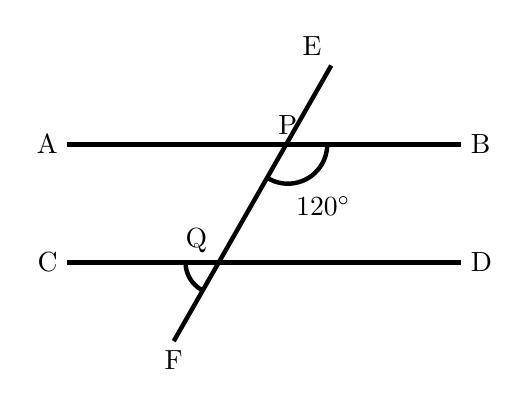
\begin{tikzpicture}

% Define points for horizontal lines
\coordinate (A) at (0, 1.5);
\coordinate (B) at (5, 1.5);
\coordinate (P) at (2.8, 1.5);

\coordinate (C) at (0, 0);
\coordinate (D) at (5, 0);
\coordinate (Q) at (1.9, 0);

% Transversal endpoints
\coordinate (E) at (3.35, 2.5);
\coordinate (F) at (1.35, -1);

% Draw horizontal lines
\draw[ultra thick] (A) -- (B);
\draw[ultra thick] (C) -- (D);

% Draw transversal
\draw[ultra thick] (E) -- (F);

% Labels for points
\node[left] at (A) {A};
\node[right] at (B) {B};
\node[above left] at (E) {E};
\node[above] at (P) {P};

\node[left] at (C) {C};
\node[right] at (D) {D};
\node[above left] at (Q) {Q};
\node[below] at (F) {F};

% Arc for angle QPB = 120° at P (from PQ direction to PB direction)
\draw[ultra thick] ($(P)+(-120:0.5)$) arc (-120:0:0.5);
\node at ($(P)+(-60:0.9)$) {$120^{\circ}$};

% Arc for angle CQF at Q (from QC direction to QF direction)
\draw[ultra thick] ($(Q)+(180:0.4)$) arc (180:240:0.4);

\end{tikzpicture}
\end{document}